%!TEX root = ../thesis.tex
\newchap{Theoretical framework}\label{sec:TH}
\minitoc
\section{The Standard Model of particle physics}

The Standard Model of particle physics (SM) is a quantum field theory that describes all the fundamental forces known beside gravity: the electromagnetic, the strong and the weak force. \\
A quantum field theory (QFT) is a framework that combines quantum mechanics, classical field theory and special relativity, allowing us to describe a particle as the excitation of a quantum field or, more formally, with an irreducible representation of the Poisson group that is characterized by its mass, spin, and additional quantum numbers.
Such theories are characterized by a Lagrangian density $\Lg{}$ that must be Lorentz invariant, must respect locality and must be renormalizable, \ie the perturbative expansions of the amplitudes must converge. \\
In the SM, additional local symmetries (Gauge symmetries) are imposed to describe the interactions between particles and for each (global) symmetry, according to the Noether theorem \cite{NoetherInvarianteVariationsprobleme}, a conserved charge arises.

\subsubsection*{Particles of the Standard Model}
Particles are divided into two main categories: fermions and bosons. 
Fermions are particles with half integer spin that obey to the Fermi-Dirac statistics and to the Pauli principle. 
Furthermore, each fermion has an antiparticle with the same mass but opposite quantum numbers.\\
Bosons are particles with integer spin that obey the Bose-Einstein statistics. In the SM there are the vector bosons (spin 1), the mediators of the forces, and the Higgs boson, the only scalar boson of the SM (spin 0). All the particles of the SM and their properties are summarized in \Fig{fig:SMpart}.



\begin{figure}[h!]
    \centering
    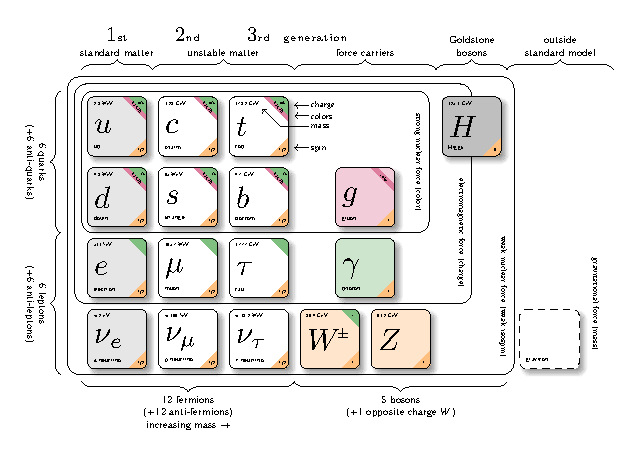
\includegraphics[width=1\linewidth]{fig//chap02-theory/sm-particles.pdf}
    \caption{Fundamental particles of the Standard Model \cite{BurgardCarstenStandardExample}}
    \label{fig:SMpart}
\end{figure}

\subsection{Gauge theories and the QED}
\paragraph*{Fermion free fields}
The Lagrangian (density) for a free fermion field is the Dirac Lagrangian

\begin{equation}\label{eq:Dirac}
\mathcal{L}_{\text{Dirac}}=i\bar{\psi}\gamma^{\mu}\partial_{\mu}\psi-m\bar{\psi}\psi
\end{equation}

where $\aff{\psi}{}=\ff{\psi}{}^\dagger\gamma^0$ is the adjoint Dirac spinor, and $\gamma^\mu$ are the 4 Dirac matrices that obey the Clifford algebra $\{\gamma^\mu,\gamma^\nu\}=2\eta^{\mu\nu}$
\paragraph*{Gauge theories}
The standard procedure to introduce a global symmetry in the Lagrangian and a Gauge boson field is the following:
\begin{enumerate}
    \item Introduce a local symmetry based on a Lie group:
    \begin{equation}\label{eq:spinor_gauge}
        \psi(x) \to \psi^\prime (x)=g(x) \psi(x) = e^{i \alpha_a(x) t^a}\psi(x)
    \end{equation}
    where $g(x)$ is a representation of the group and $t^a$ its generators
    \item Replace the partial derivatives $\partial_\mu$ with the covariant derivative $D_\mu$
    \begin{equation}\label{eq:covariant_derivative}
        D_{\mu}\psi(x)=\left(\partial_{\mu}-i g\,A_{\mu}^{a}(x)\,t^{a}\right)\psi(x)\;
    \end{equation}
    where $g$ is the coupling constant between the fermion field and the gauge fields and $A^a_\mu$ the Gauge fields 
    \item The covariant derivative should transform according to the gauge group $D_\mu \psi(x)\to g(x) D_\mu \psi(x)g^\dagger (x)$ and with some calculation, it is possible to find that the Gauge filed transform as the following under the action of the Gauge group
    \begin{equation}\label{eq:gauge_field_transformation}
        A_{\mu}(a)\rightarrow g(x)\left(A_{\mu}(x)+\frac i g\,\partial_{\mu}\right)\,g^{\dagger}(x)
    \end{equation}
    where $A_\mu=A_\mu^a(x)t^a$
    \item The final Lagrangian now has a global invariance for the Gauge group and for the Noether Theorem there is a conserved charge. Furthermore, in this procedure, another vector massless field arises.
\end{enumerate}
\paragraph*{Quantum electrodynamics}
The simplest case of a Gauge theory is the quantum electrodynamics (QED) in which the Gauge group is \U{1}, an Abelian group, \ie a commutative group ($g(x)g(y)=g(y)g(x)$)\\
The fundamental representation of the \U{1} group is $g(x)=e^{i \alpha(x)}$, \ie a local phase.\\
Imposing the \U{1} invariance on the Dirac Lagrangian (\Eq{eq:Dirac}), we obtain the QED Lagrangian (\Eq{eq:QED}).\\
In the SM, all the fermions, except the neutrinos, have an electric charge and are involved in the electromagnetic interaction.
\begin{equation}\label{eq:QED}
    \Lg{QED}=i\bar{\psi}\gamma^{\mu}(\partial_{\mu}+i q A_{\mu})\psi-m\bar{\psi}\psi-\frac{1}{4}F^{\mu\nu}F_{\mu\nu}
\end{equation}
where $A_\mu$ is the photon field, $q$ the elementary electron charge and $F_{\mu\nu}=\partial_\mu A_\nu-\partial_\nu A_\mu$ the electromagnetic tensor \\


\subsection{Quantum chromodynamics}

\subsection{Electroweak theory}

\subsubsection*{Cabbibo-Kobayashi-Maskawa matrix}

\subsection{The Higgs mechanism}

\section{The $V_{cb}$ element}

\subsection{Measurement with B mesons semileptonic decays}

\subsubsection*{Inclusive measurement}

\subsubsection*{Exclusive measurement}
